\section{Metrics}
\label{sec:metrics}

%A description of the metrics that will form the basis for evaluation. We require at least one of these to be quantitative metrics, but we are very open-minded about which ones you choose. In requiring this, we are not saying that all work in NLU needs to be evaluated quantitatively, but rather just that we think it is a healthy requirement for our course.

We measure our model performance using the accuracy metric. As shown in Table \ref{table:labeldistribution}, our dev and test sets have a uniform distribution across all the three labels. We believe this justifies using accuracy as the evaluation metric.

\begin{table*}
\small
\centering
\begin{tabular}{l ccccccc | c c}

\toprule
																														System
                                        & \multicolumn{7}{c|}{Training Data Ratio Used} 
                                        & \multicolumn{1}{c}{Dev Acc}   
                                        & \multicolumn{1}{c}{Test Acc} \\ 
                                        
																														& MNLI      & MRPC  		& QQP			&STSB		&QNLI    	& RTE		& WNLI   	& MNLI-(m/mm)   & ANLI-A1  \\
\midrule
Random    																									& 1.0       & - 		& - 			& -			& - 			& -			& -				& 33.8 / 33.2   & 33.3 \\
Baseline    																								& 1.0       & - 		& - 			& -			& -				& -			& -				& 50.3 / 49.6   & 28.9 \\
BERT\textsubscript{BASE}    		    												& 1.0       & - 		& - 			& -			& -				& -			& -				& 84.1 / 84.4   & 26.0 \\
RoBERTa\textsubscript{BASE}            											& 1.0       & - 		& - 			& -			& -				& -			& -				& 87.7 / 87.6   & 28.5 \\
RoBERTa\textsubscript{LARGE}            										& 1.0       & - 		& - 			& -			& -				& -			& -				& 92.0 / 90.0   & 46.0 \\
\midrule
\multirow{3}{*}{\shortstack[l]{BERT\textsubscript{BASE} \\ (weak supervision)}}	   		    				
																														& 0.1 			& 0.1 	& 0.1 		& -			& -				& -			& -				& 76.9 / 77.2		& 23.2 \\
																														& 0.1 			& 0.1 	& 0.1 		& 0.1		& 0.1			& 0.1		& 0.1			& 77.3 / 77.6		& 25.8 \\
																														& 1.0 			& 1.0 	& 1.0 		& 1.0		& 1.0			& 1.0		& 1.0			& 84.5 / 83.8		& 27.1 \\
\midrule
\multirow{3}{*}{\shortstack[l]{RoBERTa\textsubscript{BASE} \\ (weak supervision)}}	 
																														& 0.1 			& 0.1 	& 0.1 		& -			& -				& -			& -				& 83.6 / 84.1		& 26.0 \\  		    				
																														& 0.1 			& 0.1 	& 0.1 		& 0.1		& 0.1			& 0.1		& 0.1			& 83.6 / 84.3		& 29.3 \\
																														& 1.0 			& 1.0 	& 1.0 		& 1.0		& 1.0			& 1.0		& 1.0			& 87.5 / 87.5		& 31.3 \\
																														

\bottomrule
\end{tabular}
\caption{\label{table:accuracy} Evaluation results on the Dev/Test sets}
\end{table*}

%----------------------

\begin{table}
\small
\centering
\begin{tabular}{lcc}

\toprule
Categories			& BERT\textsubscript{BASE}   	& RoBERTa\textsubscript{BASE}   \\
\midrule
Contradiction		& 369   & 353 \\
Entailment   		& 303   & 308 \\
Neutral    			& 328   & 339 \\

\bottomrule
\end{tabular}
\caption{\label{table:predictedlabeldistribution} Distribution of predicted labels on ANLI-A1. Models trained on MNLI only.}
\end{table}


\begin{figure}
\centering
%\includegraphics[width=\textwidth,height=8cm]{SpanDetection.jpg}
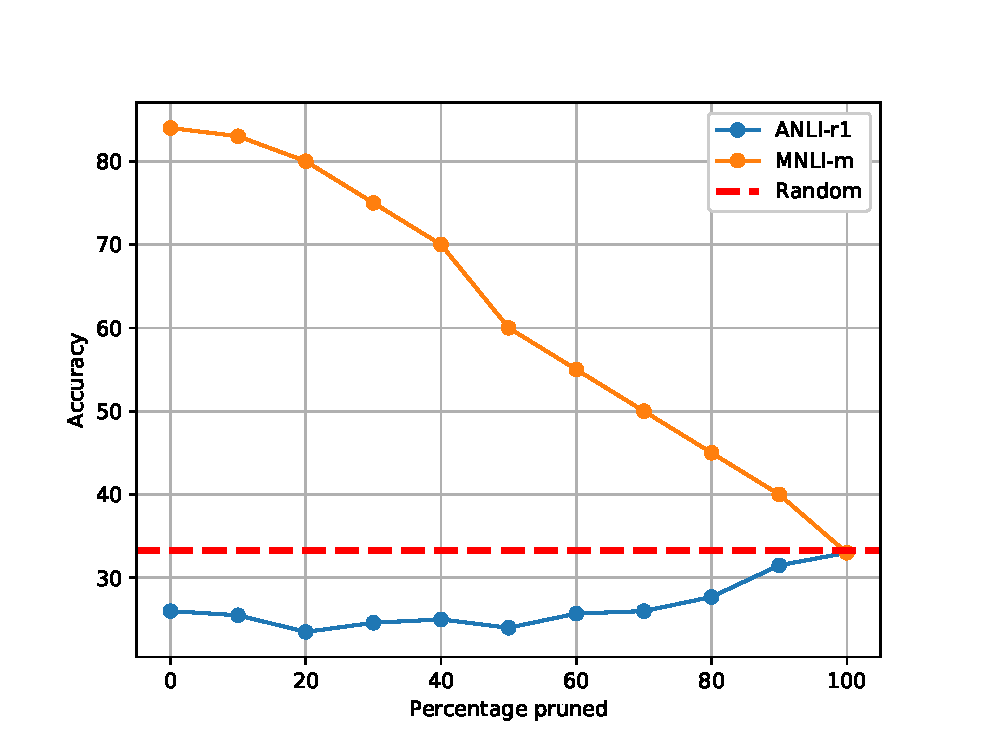
\includegraphics[width=7cm, height=5cm]{Figs4Paper/percentage_pruned_vs_accuracy.eps}
\caption{\label{fig:attentionheads} Accuracy as a function of attention heads. BERT\textsubscript{BASE} model trained on MNLI only.}
\end{figure}


%----------------------

\begin{table*}
\small
\centering
\begin{tabular}{p{5cm}p{3cm}lll}

\toprule

\textbf{Premise} & \textbf{Hypothesis} & \textbf{gold\_label} & \textbf{BERT\textsubscript{BASE} } & \textbf{RoBERTa\textsubscript{BASE} } \\

\midrule
{Julian Peter McDonald Clary (born 25 May 1959) is an English comedian and novelist. Openly gay, Clary began appearing on television in the mid-1980s and became known for his deliberately stereotypical camp style. Since then he has also acted in films, television and stage productions, and was the winner of \"Celebrity Big Brother 10\" in 2012.}        
& {Born on May 25, 1958 Julian Clary knew he would be gay.}           
& {contradiction}            
& {entailment}     
& {entailment}        \\

%\midrule
%{A French sauce spoon or saucier spoon is a spoon that is typically the size and shape of a dessert spoon, but with a flattened bowl that has a thinner edge and a small notch on one side. As the name suggests, a French sauce spoon is used to eat the sauce accompanying a dish. Such a spoon may be referred to simply as a sauce spoon, but this can also refer to a spoon used to serve sauce.}        
%& {A French sauce spoon is also called a saucy spoon.}           
%& {contradiction}            
%& {entailment}     
%& {entailment}        \\

\midrule
{Bassingham is a village and civil parish in the North Kesteven district of Lincolnshire, England. The population of the civil parish at the 2011 census was 1,425. The village is situated approximately 8 mi south-west from the city and county town of Lincoln.}        
& {Bassingham is a village and civil parish in the North Kesteven district of Lincolnshire, England and only has 1,435 citizens as of the 2011 census.}           
& {contradiction}            
& {neutral}     
& {neutral}        \\

%\midrule
%{Bimbo (also, Bimo) is the capital of Ombella-M'poko, one of the 14 prefectures of the Central African Republic, and is located 25.5 km by road southwest of the centre of the capital, Bangui. The country's second-largest city, Bimbo had a population of 124,176 as of the 2003 census and a calculated 2013 population of 267,859.}        
%& {Bimbo's population didn't quite double between 2003 and 2013.}           
%& {contradiction}            
%& {neutral}     
%& {neutral}        \\

\midrule
{Idrees Kenyatta Walker (born February 1, 1979) is a former professional American football player who was an offensive tackle in the National Football League (NFL) for six seasons. Walker played college football for the University of Florida. A first-round pick in the 2001 NFL Draft, he played professionally for the Tampa Bay Buccaneers of the NFL.}        
& {Kenyatta Walker did not play football at Florida State.}           
& {entailment}            
& {contradiction}     
& {contradiction}        \\

%\midrule
%{The Base 2: Guilty as Charged is a 2000 action/adventure film written by C. Courtney Joyner and Jeff Albert, produced Dana Dubovsky and Mark L. Lester, directed by Mark L. Lester and starring Antonio Sabato Jr. and James Remar. It is also the sequel to the 1999 film \"The Base\".}     
%& {The Base 2: Guilty as Charged was made after 1999}      
%& {entailment}            
%& {contradiction}     
%& {contradiction}        \\

\midrule
{The 2005 Big East Men's Basketball Championship was played from March 9 to March 12, 2005. The tournament took place at Madison Square Garden in New York City. The Syracuse Orange won the tournament and were awarded an automatic bid to the 2005 NCAA Men's Division I Basketball Tournament.}        
& {The tournament took place over four days.}           
& {entailment}            
& {neutral}     
& {neutral}        \\

%\midrule
%{Mountain Moonlight is a 1941 American comedy film directed by Nick Grinde and written by Mauri Grashin, John W. Krafft, Dorrell McGowan and Stuart E. McGowan. The film stars Leon Weaver, Frank Weaver, June Weaver, Betty Jane Rhodes, John Archer and Kane Richmond. The film was released on July 12, 1941, by Republic Pictures.}     
%& {Mountain Moonlight was written by several people including a man and a woman that have the same last name.}      
%& {entailment}            
%& {neutral}     
%& {neutral}        \\

\midrule
{Puss in Boots is an action game based on the DreamWorks Animation SKG movie of the same name. It was developed by Blitz Games, and released by THQ on October 25, 2011 for Xbox 360, PlayStation 3, Wii and Nintendo DS. It features support for Kinect and PlayStation Move on the respective platforms. It was released on October 25, 2011 in North America and December 2 for Europe.}        
& {Dreamworks released a movie in 2012}           
& {neutral}            
& {contradiction}     
& {contradiction}        \\

\midrule
{Binani Industries Ltd is an Indian business group based in Mumbai. It is a 143-year old business conglomerate and belongs to the legendary Braj Binani Group. The business portfolio of Binani Industries includes sectors like cement, zinc, glass-fiber, and downstream composite products.}        
& {Braj Binani Group has enjoyed ownership of Binani Industries Ltd since its creation.}           
& {neutral}            
& {entailment}     
& {entailment}        \\

\bottomrule

\end{tabular}
\caption{\label{table:erroranalysis} Examples where \textit{both} BERT\textsubscript{BASE} and RoBERTa\textsubscript{BASE} are wrong, while being in perfect agreement with each other. Models trained on MNLI only.}
\end{table*}